\documentclass[11pt,a4paper]{article}
\usepackage[T1]{fontenc}
\usepackage[utf8]{inputenc}
\usepackage[margin=25mm]{geometry}
\usepackage{lmodern,microtype,amsmath,amssymb,booktabs,tabularx,graphicx}
\usepackage[numbers,sort&compress]{natbib}
\usepackage{listings,xcolor}
\usepackage[hidelinks]{hyperref}
\usepackage{enumitem}
\setlist{nosep}
\setlength{\emergencystretch}{2em}
\lstset{basicstyle=\ttfamily\small,columns=fullflexible,breaklines=true,
  frame=none,keepspaces=true,showstringspaces=false}
\makeatletter
\let\inputtable\@@input
\makeatother
\newcommand{\code}[1]{\texttt{#1}}
\newcommand{\status}[1]{\textsf{#1}}
\title{Executable engineering arguments with EAL/2:\\
  Typed evidence, defeasible assessment and API load-test pilots}
\author{}
\date{Review manuscript for the Journal of Systems and Software\\25 September 2026}
\begin{document}
\maketitle
\begin{abstract}
Engineering decisions made with language models require a traceable relation between a claim, its observations and the rule used to interpret them. EAL/2 represents these relations in a domain-specific language and evaluates them through a Python host. The host binds typed propositions to scoped, dated evidence, invokes versioned reasoning methods and computes grounded acceptance with objections. We describe the implemented semantics and demonstrate an API performance argument. Reanalysis of a development experiment preserves 1,200 assignments across 40 controlled HTTP cases, six model snapshots and five prompting/tool conditions: 628 completed, 131 failed and 441 were unattempted. GPT-4.1 full achieved 40/40 correct assignments with EAL/MCP and 36/40 with a JSON prompt; mini achieved 32/40 and 21/40. All four full-model JSON discrepancies concerned failed-check enumeration; its decision statuses were correct. A separately analysed nano-only follow-up added ordinary deterministic validation and changed the answer schema. Plain-validator scored 11/40 against EAL/MCP's 3/40. Of the 40 EAL assignments, 13 completed incorrectly, 14 exhausted the model-call limit and ten were unattempted after a provider error stopped execution. Every attempted EAL trial obtained a correct checked packet. These pilots establish neither a notation advantage nor an accuracy advantage over ordinary validation. They provide reproducible evidence of failures in operation formatting and communication of deterministic results, within purposive cases and incomplete execution.
\end{abstract}
\noindent\textbf{Keywords:} engineering argumentation; domain-specific languages; evidence provenance; grounded semantics; language models; software performance assessment

\section{Introduction}
\label{sec:intro}
An engineering claim can be syntactically well formed and numerically plausible while referring to the wrong deployment, an expired observation or an untested assumption. A language model asked to assess that claim must select evidence for the specified deployment and interval, apply the intended rule and communicate the result without changing its scope. Producing a structured answer addresses only part of this task. The relation between the answer and the underlying observations needs an executable definition.

EAL/2, the Engineering Argument Language, makes that relation explicit. A source document names claims, evidence, assumptions, reasoning methods, supporting arguments and objections. A host validates the document, obtains observations through configured collectors, applies computational methods and returns an assessment with diagnostics. Authors can express a proposition using a typed quantity, unit, subject, scope, interval, query and result condition. Those fields constrain which observation may support the proposition. Free-text descriptions remain available for explanation, with an explicit indication that their meaning has not been verified.

The engineering contribution is the combination of these checks in a small executable system. It is useful when an assessment must be repeated after evidence changes or when a reviewer needs to distinguish a failed requirement from evidence that cannot establish whether the requirement holds. Existing work supplies argumentation semantics, structured assurance representations and model-to-solver techniques. EAL/2 adopts parts of that foundation and defines an operational profile for dated engineering observations and a tool-accessible assessment host.

Two forms of evidence support the account. Source inspection and automated tests establish behaviour of package version 2.5.0. Two supplied archives record a five-condition development experiment and a later nano-only experiment that adds ordinary validation. Each contains actual model calls and HTTP observations, together with failed and unattempted assignments. Their source snapshots, scorers and results are preserved separately. The later experiment changes both the answer schema and execution rules, so its outcomes cannot be pooled with the earlier results or treated as a controlled replication.

The paper addresses three questions. First, which relations between a proposition and an observation does the implementation check, and where does its assurance end? Second, what outcomes did the historical EAL/MCP and comparator systems produce on the assigned cases? Third, which recorded failures identify concrete changes to assessment interfaces or experimental controls? The pilot supports descriptive answers to the latter questions. It does not estimate a general advantage of a notation, establish a model-size effect or measure performance in production services.

\section{Related work and design position}
\label{sec:related}
Dung's abstract argumentation framework represents arguments and attacks and defines acceptable sets through their defence relations \citep{dung1995}. Its grounded extension provides a conservative basis for acceptance when attacks remain unresolved. EAL/2 implements an explicit attack-only solver and also a composed evaluator in which argument nodes depend on premise claims and claim nodes have alternative derivations. The composed evaluator therefore requires rules for both support and attack; attaching a familiar argumentation label to an arbitrary dependency graph would be insufficient.

ASPIC+ constructs arguments using strict and defeasible rules and supports attacks and preferences \citep{modgil2014}. EAL/2 has named arguments, objections and computational reasoning methods, but the implemented profile does not claim the full ASPIC+ semantics. Its local usability checks and acceptance equations are stated in Section~\ref{sec:semantics}. This restricted account makes the implementation's commitments testable without implying that every property of a broader structured-argumentation formalism transfers to it.

The Structured Assurance Case Metamodel defines representations for assurance claims, arguments and evidence and their interchange \citep{omg2023}. EAL/2 addresses a narrower implementation problem: repeatedly evaluating designated evidence and argument dependencies through executable methods. The comparison concerns the scope of this implementation; assessing execution in other assurance-case tools would require examining those tools individually. A representation of a supporting relation and an implementation that evaluates a particular relation provide different kinds of evidence for a software decision.

Program-aided language models delegate computations in generated programs to an interpreter \citep{gao2023}. Logic-LM translates problems into formal representations, invokes symbolic solvers and interprets the results \citep{pan2023}. These systems establish the relevance of external computation to model-assisted reasoning. EAL/2 similarly delegates defined computations, while adding evidence identity, freshness and objection handling. A solver's result remains conditional on the supplied formalisation and observations; it does not establish that an informal engineering problem has been represented correctly.

Grammar-constrained decoding studies whether generated outputs conform to a formal grammar and how that affects logical parsing \citep{raspanti2025}. The pilot reported here supplied EAL source to the model and used a common text-based operation adapter. It consequently measures neither EAL authoring ability nor grammar-constrained generation. Its JSON condition supplied a semantically corresponding argument as prompt text; it did not invoke a provider's structured-output feature.

The implementation follows conventional language-engineering separation between parsing, intermediate representation, name resolution and evaluation \citep{parr2009}. This separation permits syntax and reference errors to be reported before evidence is assessed. The host exposes tools through the Model Context Protocol (MCP) \citep{mcp2025}. MCP supplies the interaction format; the EAL implementation supplies the meanings of validation, collection and assessment. These protocol and semantic responsibilities must remain distinguishable when interpreting a successful tool call.

\section{Language and implementation}
\label{sec:language}
\subsection{Source records and assessment responsibilities}
EAL/2 source declares an environment, tools, evidence, assumptions, reasoning records, claims, arguments and objections. Patterns can generate repeated argument structures. An argument refers to a conclusion, a reasoning record and any evidence, assumptions or premise claims it needs. An objection is evaluated as an argument that attacks a designated target. Several arguments may independently offer derivations of the same claim, while the premises within a particular derivation must all hold.

The Python implementation parses the source with an ANTLR grammar and constructs a resolved intermediate representation. Validation checks identifiers, reference kinds, required fields, method-specific inputs and the acyclicity of ordinary premise dependencies. Resource limits bound processing: source input is limited to 1 MiB, token count to 100,000, records to 4,096, premise nesting to 128 and pattern applications to 1,000. The composed assessment graph admits at most 4,096 argument nodes, 4,096 claim nodes and 131,072 relationships. These bounds specify the admitted inputs to this implementation.

The package requires Python 3.11 or later. The inspected version uses ANTLR runtime 4.13.2 and MCP SDK 1.30.0, with an MCP stdio profile dated 2025-11-25. Package version, language revision and protocol profile identify different artefacts. Reproducing an assessment also requires the source document, method identifiers, collected records and assessment time. The software and data availability statement specifies the source snapshots used for the software description and historical results.

\subsection{Evidence collection, identity and time}
The host executes collectors configured by its operator. Source documents name tools and inputs; they do not supply an arbitrary executable command. Collector outcomes, including errors, are recorded in SQLite. A record can contain a collection time, content digest, metadata and a structured value used by a reasoning method. Its digest checks content consistency against the recorded value. It cannot establish that a sensor was calibrated, that a remote service was honest or that the observation represents the intended operational population.

Freshness is evaluated against an explicit assessment time. If $t$ is that time, $t_c$ the recorded collection time and $a$ the permitted age, the condition is
\begin{equation}
  0 \leq t-t_c \leq a.
  \label{eq:freshness}
\end{equation}
Preserving the original collection time when importing evidence prevents ingestion from making an old observation fresh. Assumption validity uses a declared interval with an inclusive start and an exclusive end. These temporal checks establish eligibility under the declared rules. They cannot establish that the measured system remained unchanged throughout the interval.

\subsection{Typed propositions and computational methods}
\label{sec:typed}
A typed proposition identifies a subject $s$, quantity $q$, unit $u$, scope $\sigma$, interval $I$, query $Q$ and result predicate $R$. A designated computational evidence value carries an \code{EAL/typed-input/1} envelope. The host checks that its method, subject, quantity and scope match the proposition, that its unit is compatible, that its observation interval contains $I$, and that the query agrees under canonical comparison. The method then computes a result for evaluation against $R$.

Figure~\ref{fig:typed} illustrates these correspondences with stipulated pressure observations. The unit conversion allows a result expressed in pascals to be compared with a condition in kilopascals. Agreement of the metadata is necessary for this binding, but matching an authored scope string does not independently verify experimental assignment. The figure illustrates a computational interface using stipulated values.

\begin{figure}[tbp]
  \centering
  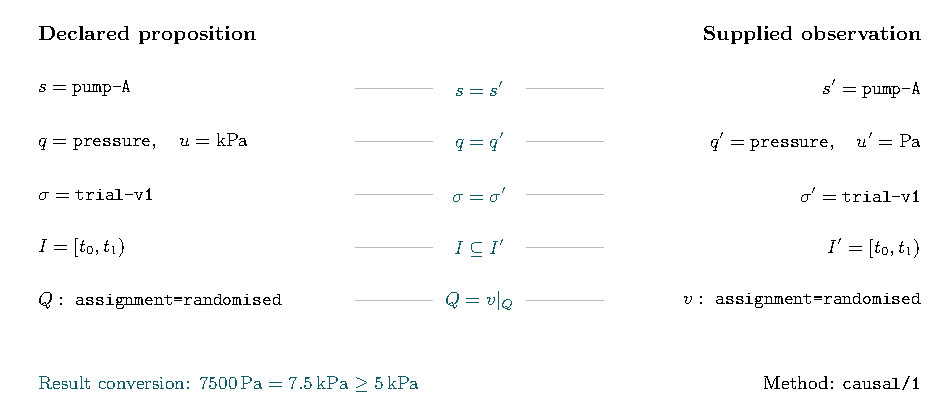
\includegraphics[width=160mm]{figures/typed-correspondence.pdf}
  \caption{Typed correspondence for a constructed \code{causal/1} example. The two columns denote proposition fields and supplied observation fields; connecting relations specify the checks. The observation interval must contain the proposition interval, and $v|_Q$ denotes the fields of the supplied value selected by the query. Compatible units permit the illustrated conversion before the result condition is checked. The values are stipulated, and the declared randomised assignment is not independently established by this correspondence.}
  \label{fig:typed}
\end{figure}

Eight built-in method families are versioned separately from their display names. The default \code{structured/1} method checks the availability of declared dependencies while retaining an authored rationale. It does not turn that rationale into a formal entailment. \code{deductive/1} evaluates bounded propositional inputs, with at most 12 atoms, and checks premise consistency. \code{inductive/1} uses a Wilson interval; \code{abductive/1} uses declared priors and likelihoods; and \code{causal/1} evaluates a contrast between independent groups. \code{counterfactual/1} operates on a bounded affine structural causal model with fixed exogenous inputs. \code{analogical/1} compares specified features, and \code{temporal/1} checks sampled temporal coverage. Each method's result is conditional on its input schema and assumptions. In particular, sampled temporal coverage does not prove continuous-time behaviour, and a group contrast alone does not identify an intervention effect.

A registered custom method can extend the computations. Resource-limited worker execution bounds some failures, but it does not make custom code a security sandbox or prove its purity. Method registration and collector configuration remain trusted host responsibilities. The assessment includes \code{prose\_verified: false} to identify the separate status of explanatory prose. A reader can inspect what was computed without treating the surrounding natural-language interpretation as mechanically proved.

\section{Defeasible assessment and implementation evidence}
\label{sec:semantics}
\subsection{Acceptance of arguments and claims}
Let $N$ be the finite set of argument and objection nodes and $C$ the finite set of claims. For $n\in N$, let $U(n)$ denote the result of its local usability checks, $P(n)\subseteq C$ its required premise claims and $T(n)\subseteq N$ its attackers. For $c\in C$, let $D(c)\subseteq N$ contain its derivations. Labels range over accepted, rejected and undecided. With $\mathsf{A}$ and $\mathsf{R}$ denoting the first two labels, the evaluator applies the following rules:
\begin{align}
 n:\mathsf{A} &\quad\text{if } U(n)\land
       \bigwedge_{p\in P(n)}p:\mathsf{A}\land
       \bigwedge_{b\in T(n)}b:\mathsf{R}, \label{eq:accept}\\
 n:\mathsf{R} &\quad\text{if } \neg U(n)\lor
       \bigvee_{p\in P(n)}p:\mathsf{R}\lor
       \bigvee_{b\in T(n)}b:\mathsf{A}, \label{eq:reject}\\
 c:\mathsf{A} &\quad\text{if } \bigvee_{d\in D(c)}d:\mathsf{A}, \label{eq:claimaccept}\\
 c:\mathsf{R} &\quad\text{if } \bigwedge_{d\in D(c)}d:\mathsf{R}. \label{eq:claimreject}
\end{align}
Empty conjunctions are true and empty disjunctions false. Thus a claim with no derivation is rejected by the graph evaluator. This graph label means that no accepted derivation is available; it does not establish the factual negation of the engineering claim.

Evaluation starts with every label undecided and repeatedly applies the rules until no label changes. Settled labels are retained. On a finite graph, this monotone accumulation of information terminates because each node and claim can become settled at most once. This argument concerns termination of the label computation after local checks have completed. Collector execution and custom methods require their own runtime controls.

The rules make conjunctive premises and alternative derivations explicit. An accepted premise alone cannot compensate for another rejected premise of the same argument. An accepted alternative derivation can support a claim whose other derivation has been rejected. Reusing an evidence record across derivations does not create independent observations or multiply the statistical strength of that evidence. Attack cycles may remain undecided even though ordinary premise dependencies are acyclic.

The public engineering statuses include \status{supported}, \status{contested}, \status{unsupported} and \status{out\_of\_scope}. They are interpretations of an assessment in its declared environment. Evidence availability, graph acceptance and the truth of an external proposition are separate quantities. An application that needs an \status{unavailable} decision category must specify its mapping from diagnostics and evidence checks; Section~\ref{sec:protocol} describes the historical experiment's mapping.

\subsection{What the tests establish}
The repository checks the attack-only solver against independent complete-extension enumeration for all 531 directed graphs with zero to three nodes, including self-attacks. The composed evaluator is compared with an independent Dung translation over 1,024 two-node, one-claim combinations, 200 seeded larger cases and 512 three-node attack-only cases. Additional tests exercise propagation through a chain of 4,096 argument nodes and 4,096 claims across 8,192 rounds. These finite comparisons check the implemented rules on the enumerated and generated inputs; they are not a mechanised proof covering every graph within the resource limits.

For the source snapshot described in this paper, the full test suite completed with 846 passing tests. It includes parser, validation, evidence, reasoning, command-line and MCP interaction tests. Agreement between an implementation and a translated reference could still reflect a shared modelling error, so the equations, independent enumerations and executable tests are supplied together. Test success establishes the checked software behaviour. It cannot establish that a deployed collector observes the intended system or that a language model will communicate an assessment faithfully.

\section{Worked API performance argument}
\label{sec:example}
The repository's worked example concerns a named API service, build, load-test run and concurrency level. A collector validates the report and computes request count, nearest-rank sample p95 latency and the proportion of failed requests. For $n$ ordered latency values $x_{(1)},\ldots,x_{(n)}$, the sample quantile is
\begin{equation}
 \widehat q_{.95}=x_{(\lceil .95n\rceil)},\qquad
 \widehat e=\frac{\#\{\text{failed requests}\}}{n}.
 \label{eq:metrics}
\end{equation}
The declared acceptance conditions are $n\geq100$, $\widehat q_{.95}\leq200$ ms and $\widehat e\leq0.01$. Report identity, completeness, freshness and internal consistency must also satisfy their checks. These thresholds specify a decision for a finite report; they do not provide a confidence statement about a service's long-run tail latency or error probability.

The example supplies synthetic records with 100 requests, a sample p95 of 180 ms and one failed request. It is assessed at a fixed time, with a maximum evidence age of 86,400 seconds. The inclusive inequalities admit the error rate of exactly 1\%. Figure~\ref{fig:region} shows the acceptance region conditional on sufficient request count and eligible evidence. Its second marked point stipulates two failures, making the report fail the error-rate condition while leaving the latency value unchanged. This perturbation illustrates the rule without adding a measured observation.

Listing~\ref{lst:example} reproduces the claim and argument from the executable example. Its collector computes the metrics, and the evidence declaration applies the three thresholds. The reasoning record selects \code{structured/1}. Consequently, this example demonstrates executable evidence requirements and dependency assessment with an authored rationale; it does not exercise the typed proposition binding illustrated in Figure~\ref{fig:typed}. The complete source and its collector are included in the repository and covered by the test suite.

\lstinputlisting[firstline=32,lastline=41,caption={Claim and argument excerpt from \code{examples/api-load-test/source.eal}. The referenced environment, reasoning and evidence records are declared earlier in that file.},label={lst:example}]{../examples/api-load-test/source.eal}

\begin{figure}[tbp]
  \centering
  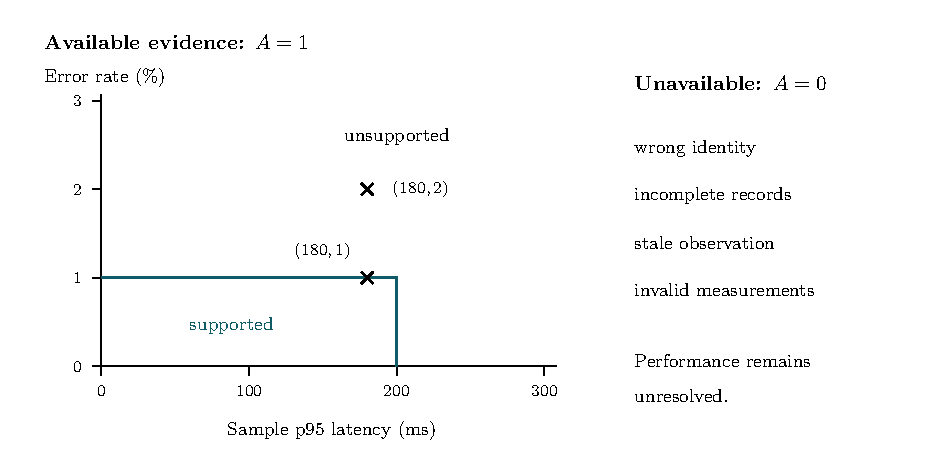
\includegraphics[width=160mm]{figures/acceptance-region.pdf}
  \caption{Decision region for the worked API example, conditional on at least 100 requests. With eligible evidence ($A=1$), the inclusive bounds are sample p95 latency at most 200 ms and error rate at most 1\%. The point $(180,1)$ uses the synthetic example's values; $(180,2)$ is a stipulated perturbation. When report validity, identity, completeness, freshness or consistency is unresolved or fails ($A=0$), performance remains unavailable for this decision. The axes show the declared decision rule; no pilot measurements or fitted response surface are plotted.}
  \label{fig:region}
\end{figure}

Pinning the report digest and comparing command-line and MCP assessments checks whether the same example is interpreted consistently through two interfaces. A digest mismatch, stale report or different build cannot be repaired by a favourable performance number. The operational consequence is to obtain eligible observations before deciding whether the performance requirement holds. This consequence motivates the unavailable category used in the experiment.

\section{Historical pilot: materials and method}
\label{sec:protocol}
\subsection{Run identity and case construction}
The analysed artefact is GitHub Actions run 36163505801, attempt 1, executed on 25 September 2026 using commit \code{3490076dd78404caa1326d9aae704f964910c4c8}. Its manifest identifies plan version 2.0.0 and run schema \code{eal-api-experiment-run/2}. The supplied ZIP's SHA-256 agrees with the digest recorded for GitHub artefact 10879620453. Reanalysis uses the original reference and scoring code from that commit. It does not apply the later experiment's additional comparator or revised outcome fields to the historical answers.

The 40 cases comprise four variations in each of ten designed families: healthy, near-limit, slow, errors, incomplete, wrong identity, stale, corrupt, conflicting and distractor. Each case acquired a real HTTP workload against a controlled loopback service. The harness then constructed a report bundle, including annotated fault injections where required. The harness used the same immutable report bundle for every model and condition assigned to a case. Case identity and byte content are verified during reanalysis. This arrangement controls differences in observations across conditions while retaining a realistic report-selection task. The cases are development examples selected by mechanism, with no probability sampling of production incidents.

The independent reference recomputes metrics from raw request rows and evaluates report selection, identity and validity without calling the EAL collector. A family's intended label does not determine its reference outcome: measured rows and injected conditions do. The final reference distribution is nine supported, 12 unsupported and 19 unavailable cases. Freshness is evaluated against a shared frozen assessment time with a 300-second age limit. This differs from the worked example's one-day limit and is preserved in the historical reanalysis.

\subsection{Conditions, models and resource limits}
The assignment ledger crosses 40 cases, six model snapshots and five conditions, giving 1,200 assignments. The EAL/MCP condition supplies a complete EAL source document and access to the EAL collection and assessment host. The JSON condition supplies the corresponding argument structure as JSON prompt text, with direct collector access. Three prose conditions provide a brief instruction, explicit decision instructions or a review-oriented instruction, also with direct collector access. The historical JSON and prose conditions have no equivalent EAL checker. All conditions receive the same report catalogue and acceptance criteria. Their tools return collector-derived metrics and measurement facts from the same underlying reports; EAL/MCP additionally returns the checked assessment. Prompt lengths and available tool conclusions therefore differ. The comparison concerns these complete systems.

The EAL condition uses \code{structured/1} with the supplied argument. The pilot therefore tests report selection and communication of a computed assessment; it does not exercise model authoring, typed proposition binding or objection handling. The independent reference uses raw rows, whereas the models report metrics already computed by their collector.

The pinned GPT-4.1 nano, mini and full snapshots are all dated 2025-04-14 and use temperature 0.2. GPT-5.4 nano and mini are dated 2026-03-17; the full snapshot is dated 2026-03-05. The GPT-5.4 configurations request medium reasoning effort. These names identify the archive's provider snapshots and commercial tiers. The study supplies no parameter counts or controlled manipulation of model capacity.

All six models use the same text-based JSON operation adapter; native provider tool mode is disabled. The EAL condition connects those operations to a real MCP session, while the other conditions call the direct collector. Each trial permits at most six model calls, each with at most 4,096 output tokens and a 120-second timeout. The manifest records a USD 20 per-model admission allowance, a one-second minimum call interval, six workers and assignment seed 20260925. Equal limits do not imply equal prompt tokens or equal computational assistance. In particular, a model requesting an EAL assessment can receive a checked conclusion unavailable to a comparator model.

\subsection{Reference decisions and correctness}
\label{sec:scoring}
Let $A$ mean that report validity, identity, completeness, freshness and consistency all evaluate to true. The reference status is unavailable when $A$ is false or unresolved. Given $A$, it is supported when all three performance predicates hold and unsupported otherwise. This order prevents a missing or invalid observation from being classified as demonstrated poor performance.

The required final answer identifies the report and its scope, gives a status, enumerates failed checks and supplies request count, sample p95 and error rate. The original rubric requires collection, correct report selection, exact scope, correct status, an exact set of failed checks, exact count and latency/error metrics within 0.01 in their reported units. The narrative explanation is retained but is not scored. A failed check is a predicate whose value is explicitly false. An unknown predicate is not included in that set. The version-2 answer schema has no separate \code{unknown\_checks} field.

This distinction is consequential for corrupt reports. Their validity check can be false while other checks and metrics are unknown. Listing every unresolved check as failed violates the rubric even if the answer's unavailable status is correct. Reporting both the composite score and the underlying discrepancy is necessary to interpret such cases.

The EAL host's unsupported assessment can arise from a measured failure or from unavailable evidence. The version-2 adapter therefore supplies both \code{host\_status} and \code{decision\_status}, together with a status mapping. Its presence does not guarantee that a model will select the application-level decision status. Retained host assessments are compared with the independent reference, allowing a disagreement in the final answer to be separated from a disagreement in the host's computation. The later experiment uses one application-level \code{status} in the model-visible packet, as described in Section~\ref{sec:nano}.

\subsection{Analysis of incomplete execution}
\label{sec:analysis}
One attempt was assigned to each case--model--condition combination. The archive records 628 completed attempts, 131 failures and 441 assignments not attempted. Of the failures, 128 reached the model-call limit and three returned provider errors stating that the response was incomplete. The runner's broad provider-error rule stopped subsequent assignments for the affected model. Each GPT-5.4 snapshot encountered such an error; the full snapshot stopped after its first assignment. These stops account for all unattempted assignments.

The primary descriptive score retains the assignment denominator. Write $Y_{ima}=1$ when case $i$, model $m$ and condition $a$ completed with a correct answer, and zero otherwise. For each model and condition, the reported score is $\sum_{i=1}^{40}Y_{ima}/40$. This describes the recorded system's realised yield under the run's stopping rule. A zero caused by non-execution is not evidence of an incorrect answer that a model would have produced.

For the paired EAL/MCP--JSON contrast, let $n_{10}$ count cases correct only under EAL/MCP and $n_{01}$ those correct only under JSON. The finite-case difference is
\begin{equation}
 \Delta_m=\frac{1}{40}\sum_{i=1}^{40}(Y_{imE}-Y_{imJ})
          =\frac{n_{10}-n_{01}}{40}.
 \label{eq:delta}
\end{equation}
Completed-pair counts accompany this contrast. Conditioning on completion changes the analysed subset and may select easier cases; it cannot repair missing outcomes. No confidence interval, significance test or equivalence conclusion is assigned to these purposively constructed cases. There is one realised model attempt per assignment, shared case structure within each family and no probability sampling scheme for a target population. The observed differences are descriptive development results.

\section{Results}
\label{sec:results}
\subsection{Assignment yield and paired outcomes}
Table~\ref{tab:accuracy} reports correct assignments across all five conditions. GPT-4.1 full and mini completed all 200 assignments each; their differences therefore do not depend on unattempted cases. Full scored 40/40 in EAL/MCP and 36/40 in JSON, a difference of 10 percentage points. Mini scored 32/40 and 21/40, a difference of 27.5 percentage points. GPT-4.1 nano scored 16/40 and 6/40, but only 25 of those paired assignments completed in both conditions. Its 25-point difference combines answer correctness and completion under the specified limits.

\begin{table}[tbp]
\centering\small
\caption{Correct assignments out of 40 in each model--condition cell. Failed and unattempted assignments remain in the denominator. Snapshot dates and settings are given in Section~\ref{sec:protocol}. ``Full'' identifies the unqualified model name.}
\label{tab:accuracy}
\begin{tabular}{lrrrrr}\toprule
Model & EAL/MCP & JSON & Brief & Explicit & Review\\\midrule
\inputtable{results/accuracy-rows.tex}
\bottomrule\end{tabular}
\end{table}

Figure~\ref{fig:paired} shows the paired counts. For GPT-4.1 mini, EAL/MCP alone was correct on 12 cases and JSON alone on one; the two systems were both incorrect on seven. For full, the four discordant cases all favoured EAL/MCP under the composite rubric. These counts locate agreement and disagreement more precisely than marginal percentages alone.

\begin{figure}[tbp]
\centering
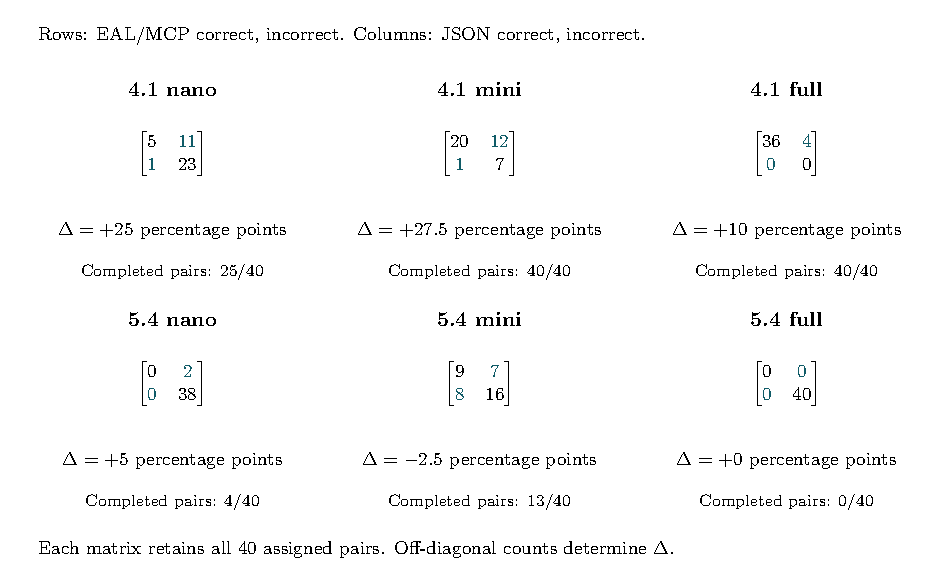
\includegraphics[width=160mm]{figures/paired-outcomes.pdf}
\caption{Paired EAL/MCP and JSON assignment outcomes. Rows are EAL/MCP correct and incorrect; columns are JSON correct and incorrect. Each matrix sums to all 40 assigned cases. The off-diagonal counts give $\Delta$ through Equation~\ref{eq:delta}; completed-pair counts disclose exposure. Here ``incorrect'' includes failed and unattempted assignments under the declared yield measure. In particular, the 40 in the GPT-5.4 full lower-right cell represents absent successful execution, not 40 observed pairs of wrong answers.}
\label{fig:paired}
\end{figure}

The GPT-5.4 records support a narrower account because model-level stopping removed substantial exposure. Mini scored 16/40 in EAL/MCP and 17/40 in JSON, with only 13 completed pairs. Nano scored 2/40 and 0/40, with four completed pairs. Full supplied no completed assignment. Table~\ref{tab:disposition} separates completion, failure and non-execution for each model. These totals preclude interpreting the GPT-5.4 scores as an ordered capability comparison with GPT-4.1.

\begin{table}[tbp]
\centering\small
\caption{Disposition of the 200 assignments for each model, pooled over five conditions. A failed attempt consumed execution; an unattempted assignment remained after stopping.}
\label{tab:disposition}
\begin{tabular}{lrrr}\toprule
Model & Complete & Failed & Not attempted\\\midrule
\inputtable{results/disposition-rows.tex}
\bottomrule\end{tabular}
\end{table}

\subsection{What the correctness differences mean}
All four incorrect JSON answers from GPT-4.1 full concerned corrupt-report cases. Their statuses, report selection, scope and metrics were correct; their failed-check sets included unknown checks. Thus the 40 versus 36 composite score supplies evidence about compliance with the answer rubric, while the observed status accuracy was 40/40 in both conditions. A claim that EAL/MCP improved full-model decision-status accuracy would misstate these data.

The eight incorrect EAL/MCP answers from GPT-4.1 mini identify a different problem. Seven had an incorrect status: two incomplete-report cases, four stale-report cases and one wrong-identity case. One further answer used the wrong scope on a healthy case. All 40 mini EAL/MCP answers had correct metrics and failed-check sets. The discrepancy between an accurate computed result and its final status expression makes status communication an interface concern, even when the model successfully obtains the relevant evidence.

Across the run, 141 host checks were recorded, and all agreed with the independent reference according to the archived comparison flags. This is an agreement rate for the checks that were actually invoked and retained; it is not coverage of all 240 EAL assignments. It supports separating the observed communication failures from failures of those recorded host computations. The reference itself remains a program subject to specification and implementation error.

\subsection{Consumption and reproducibility}
The archive records 2,342 model calls and an estimated total cost of USD 3.97892431 at the manifest's frozen token rates, with no calls missing cost accounting. Table~\ref{tab:cost} gives condition totals. They include calls from failed attempts. Missing execution reduces some totals substantially, so lower cost in an incomplete cell does not establish greater efficiency at completing the task.

\begin{table}[tbp]
\centering\small
\caption{Recorded token-cost estimates in USD, rounded to four decimal places. Rates are those frozen in the run manifest, not current prices. Zero cells have no recorded model calls.}
\label{tab:cost}
\begin{tabular}{lrrrrr}\toprule
Model & EAL/MCP & JSON & Brief & Explicit & Review\\\midrule
\inputtable{results/cost-rows.tex}
\bottomrule\end{tabular}
\end{table}

Each of the three incomplete-response errors occurred on a response reporting 4,096 output tokens, the configured cap. The archive reports 4,073 reasoning tokens for the GPT-5.4 nano response, 4,027 for mini and 38 for full. These observations identify a budget/response interaction requiring investigation. They do not establish the provider's internal stopping mechanism or predict the result of a larger budget.

The supplied reproduction script verifies the archive-derived file hashes, the 40 case hashes, all 1,200 assignment identities and the two historical scoring-module hashes. It recomputes the independent reference and rubric for all 759 attempted assignments, checks token costs against the frozen rates and regenerates the historical summary. Every recomputed score and the full summary match the archived originals. Reproduction requires no network connection or new model calls. The paper's numerical tables and paired matrices are generated from that replay, avoiding manual transcription of cell results.

\subsection{Nano-only follow-up with ordinary validation}
\label{sec:nano}
Actions run 36176588712 used plan 3.1.0 at commit \code{8220e838a8d4}. It assigned GPT-4.1 nano, snapshot 2025-04-14, to 40 cases in six conditions. The additional plain-validator condition combines explicit prose with deterministic checking through the direct collector. The revised answer schema separates \code{failed\_checks} from \code{unknown\_checks}. Both checked conditions return one application-level status. Temperature 0.2, text-mediated operations and the six-call limit remain fixed. The run reuses the case identifiers with newly acquired HTTP observations; changing observations, rubric and failure handling prevents a direct estimate of performance change from the version-2 run.

Table~\ref{tab:nano} preserves all 240 assignments. Plain-validator achieved 11/40 correct assignments, compared with 3/40 for EAL/MCP and 5/40 for explicit prose. These are differences of 20 and 15 percentage points, respectively, in realised assignment yield. Only eight EAL/MCP--validator pairs completed in both conditions. Within that selected subset, plain-validator alone was correct on three cases and EAL/MCP alone on none. The result supplies counterevidence to an EAL/MCP advantage on this task, while incomplete execution and unequal interfaces prevent attributing the difference to notation.

\begin{table}[tbp]
\centering\small
\caption{Nano-only follow-up under plan 3.1.0. Each condition has 40 assigned cases. Scores retain failed and unattempted assignments.}
\label{tab:nano}
\begin{tabular}{lrrrr}\toprule
Condition & Correct & Complete & Failed & Not attempted\\\midrule
\inputtable{results/nano-outcome-rows.tex}
\bottomrule\end{tabular}
\end{table}

The EAL/MCP assignments separate into three correct completions, 13 incorrect completions, 14 exhausted conversations and ten unattempted cases (Figure~\ref{fig:nano}). All 30 attempted trials successfully invoked the fixed EAL assessment on their first model call. Their validation, collection, reasoning and explanation receipts record success; all 34 returned packets, including repeated assessments, agree with the independent reference on the supplied measurements and decision fields. The failures therefore occur after successful assessment in these trials.

\begin{figure}[tbp]
\centering
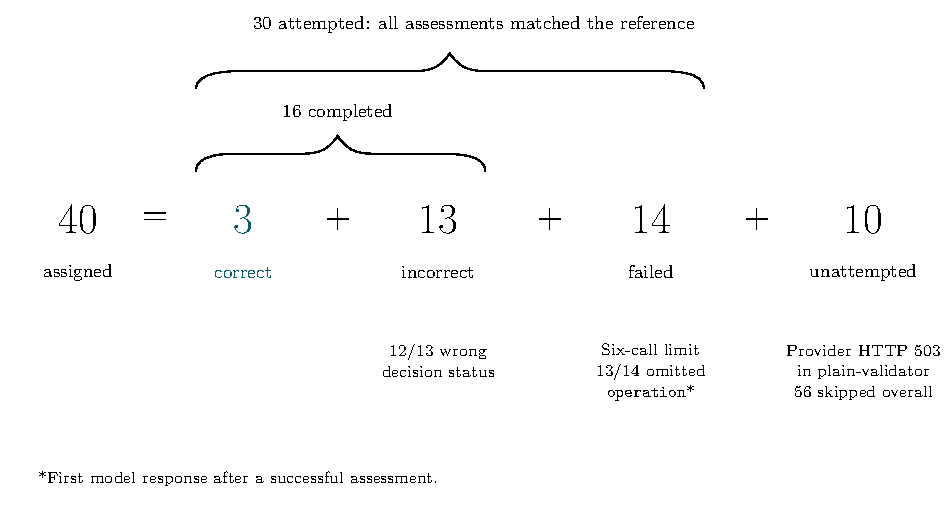
\includegraphics[width=160mm]{figures/nano-failure-diagnosis.pdf}
\caption{Disposition of the 40 EAL/MCP assignments in the nano follow-up. Every attempted assignment obtained a correct assessment packet. The nested counts distinguish incorrect final answers, exhausted conversations and assignments removed by the later model-level stop. Counts describe this execution and preserve its missing outcomes.}
\label{fig:nano}
\end{figure}

All 14 exhausted conversations used the six permitted model calls. In 13 of these, the first response after assessment omitted the required operation name; the corresponding count across all attempted EAL trials was 26/30. Later replies repeatedly omitted required fields. Two exhausted trials produced the correct scored fields but omitted the required explanation, which was a schema requirement although explanation quality was unscored. These records distinguish inability to complete the operation protocol from an incorrect engineering decision.

Among the 13 incorrect completions, 12 have a wrong status, five have wrong metrics, four have wrong failed-check sets, three have wrong unknown-check sets and one has wrong scope; these counts overlap. No completed EAL answer uses \status{unavailable}, although seven require it. In case \code{case-cd277ae1a808}, the packet reports \status{unsupported} with a 20\% error rate and a failed error-rate check. The final answer preserves those facts and explains why the run fails, yet labels it \status{supported}. Other answers replace available measurements with null after receiving a protocol error, treating a malformed operation as absent evidence. The ordinary-validator condition also mislabels unavailable evidence, so this communication problem extends beyond EAL.

The annotation claiming that all checks passed appears alongside measurements in some packets. Its repetition, prompt length and the amount of provenance may affect model behaviour, but this run does not isolate those effects. A wrong-identity EAL case with a neutral annotation and no protocol error still changes the correct \status{unavailable} packet to \status{supported}. The retained evidence establishes disregard or alteration of correct decision fields; it does not establish a single prompt feature as their cause.

The run ended when a plain-validator call returned HTTP 503. Its recorded usage and charge were unknown. The runner marked the error retryable but stopped the model under the frozen unknown-cost rule. The remaining 56 assignments, including ten EAL assignments, were never dispatched. Thus EAL non-execution was caused by a shared execution stop, while all 14 EAL failures were exhausted conversations. Across conditions, 141 assignments completed, 43 failed and 56 remained unattempted. The archive records 689 calls, USD 0.1146428 in known token costs and one call with unknown cost. This is partial cost accounting, not a claim about the provider's total charge.

The separate reproduction script verifies all retained case hashes and the eight preserved source/configuration hashes, recomputes all 184 attempted scores and reproduces the complete 240-assignment summary. It also rechecks every retained model-visible measurement packet against raw case rows. The curated follow-up data retain response text, protocol errors and full tool traces, permitting the communication and execution diagnoses to be regenerated without model calls. Neither pilot supplies an efficacy result for subsequent protocol repairs.

\section{Discussion and threats to validity}
\label{sec:discussion}
\subsection{Bounded engineering value}
The implementation makes several engineering mistakes detectable before a conclusion is communicated: an evidence record can name the wrong subject, use an incompatible unit, fall outside the permitted interval or fail a method-specific input condition. The composed evaluator also exposes unresolved attacks and unavailable premises. These checks provide inspectable reasons for an assessment. Their usefulness depends on engineers choosing quantities, intervals, collectors and methods that represent the intended question.

The pilot adds evidence about the interaction surrounding those checks. On the completely executed GPT-4.1 full and mini strata, EAL/MCP had higher composite correctness than the four supplied alternatives. However, the full-model JSON difference was entirely attributable to the exact failed-check rubric, and mini still miscommunicated seven statuses after using EAL/MCP. These findings support improving the application response schema and its interpretation. They do not establish that an executable host eliminates reasoning errors.

The nano follow-up favours ordinary validation over EAL/MCP in realised assignment yield. Together, the pilots show that providing a correct computed verdict does not ensure a correct model response. The EAL condition also changes notation, provenance and the MCP execution route, whereas the plain-validator condition uses a direct checker. A comparison with matched response content, prompt information and output requirements would distinguish these contributions. Model authoring of EAL source requires a separate task and failure taxonomy because both pilots supply the source in advance.

The accompanying protocol-4 implementation addresses the recorded failure mechanisms through explicit operation contracts. The host supplies an omitted report identifier from the most recently inspected packet and an omitted scope from the requested task; conflicting supplied fields are rejected. Explanation becomes optional, and protocol feedback distinguishes operation errors from unchanged evidence. Model finalisation remains the default and retains model-authored decisions, including incorrect ones. A separately labelled checked-finalisation mode returns the deterministic result directly for the two checked conditions; its outcomes must remain separate from model-finalised outcomes. Bounded retries for transient transport and server failures preserve unknown-charge reservations and remain within the existing call limit. These changes have offline implementation checks, with no new model-performance measurements reported here.

\subsection{Construct and internal validity}
The composite outcome combines report acquisition, selection, scope, status, failed-check enumeration and metric reporting. It deliberately demands a complete answer, but its exact-set requirement makes unknown-versus-failed wording consequential. Reporting status accuracy and error components alongside the composite score avoids equating every failed answer with a wrong engineering decision. Explanation quality, calibration, user comprehension and downstream deployment choices were not measured.

The independent reference recomputes results from raw rows, reducing direct implementation reuse with the EAL collector. Both nevertheless implement the same authored specification, and both could embody a mistaken requirement. Case construction, protocol design and interpretation occurred within the project that develops EAL. No independent participant study or external replication is available. Archive integrity and exact score reproduction address data handling; they cannot remove these design dependencies.

The model-level stopping rules make missingness depend on execution outcomes and assignment order. Treating all assignments as denominators preserves each run's operational yield but penalises conditions scheduled after a model stopped. Restricting analysis to completed trials changes that problem into selection bias. The paper therefore reports both disposition and paired completion and refrains from assigning missing counterfactual answers. Protocol 4 defines bounded retry and continuation rules prospectively; evaluating them requires a new run. Reclassifying the historical 503 response after observing its consequences would change the historical protocol.

\subsection{External and statistical validity}
The workload was a local HTTP service with controlled modifications to reports. It supplies real requests and timing observations but does not sample the operating conditions, organisational practices or failure distributions of deployed services. Four variations within each designed family share substantial structure. Forty case identifiers consequently do not imply 40 independent draws from an engineering population.

Provider snapshots, reasoning settings and per-call limits are specific to the archived run. Commercial model tiers are not experimental manipulations of a single capability variable. Cross-family differences combine architecture, training, inference behaviour and interface configuration. Single realised attempts also leave response variability unmeasured. These restrictions motivate descriptive counts and paired differences rather than population confidence intervals or claims of statistical equivalence.

The software account and the pilot concern different commits. The current package's successful test run does not retroactively validate every historical execution path, and the pilot does not measure later changes. The accompanying materials retain both identities, the original scorer and the artefact digest so that a future study can state exactly which components were changed.

\section{Conclusion}
EAL/2 provides an executable relation between typed propositions, dated evidence, reasoning methods and defeasible acceptance. Its value is clearest where an engineering assessment must reveal which observation was used, whether it met declared eligibility conditions and how an objection affected the conclusion. The implementation tests and worked example establish bounded software behaviour; they leave the adequacy of the chosen engineering formalisation open to inspection.

Reanalysis of both historical pilots reproduces their scores and preserves incomplete execution. The completely executed GPT-4.1 full and mini strata favour EAL/MCP under the earlier composite rubric, with the full-model JSON difference confined to failed-check enumeration. The later nano study favours plain-validator and locates EAL failures after successful assessment: malformed completion operations, incorrect final fields and a shared provider stop. The evidence supports executable assessment as a bounded software capability, while leaving an accuracy advantage over ordinary validation unestablished. Matched interfaces and predefined continuation rules are required to test proposed repairs.

\section*{Software and data availability}
\label{sec:availability}
Source and research materials are available in the \href{https://github.com/emmett08/earl}{\code{emmett08/earl}} repository. The implementation description and test run refer to commit \code{8220e838a8d42922edc0496ff50927c672a1f87d}. The first experiment refers to commit \code{3490076dd78404caa1326d9aae704f964910c4c8} and \href{https://github.com/emmett08/earl/actions/runs/36163505801}{Actions run 36163505801}. The \code{paper/data} directory preserves all raw case rows and the assignment, answer, outcome and token-accounting fields required for its score reproduction. It also contains hashes and provenance for the supplied archive. For that first run, full provider response text, replay handles and per-call tool transcripts remain in the original Actions artefact and are not duplicated in the curated scoring dataset. The repository records the need for durable full-archive deposits before journal submission.

The nano-only follow-up is \href{https://github.com/emmett08/earl/actions/runs/36176588712}{Actions run 36176588712}, at the implementation commit given above. Its separate \code{paper/data/nano-v3} dataset includes raw cases, all 240 assignments, provider response text without replay handles, model-visible host packets and complete tool traces. Preserved source files in \code{paper/analysis/nano\_v3\_original} are checked against the historical manifest before scoring. The two datasets retain their distinct protocols and newly acquired observations.

Running \code{make -C paper} regenerates the results, four TikZ figures and manuscript PDF. The reanalysis uses Python's standard library; figure and manuscript compilation require a LaTeX installation with TikZ, \code{standalone}, \code{natbib}, \code{latexmk} and the packages listed in the source. Author metadata and submission declarations are kept in the accompanying submission checklist for author confirmation before submission.

\bibliographystyle{plainnat}
\bibliography{references}
\end{document}
